\chapter{Datastructure Octree}
\label{mise_en_oeuvre}

\paragraph{}
Pour la gestion des collisions et l'attraction/répulsion, la recherche du plus
proche voisin est utilisée pour chaque atome et pour chaque frame. Avec la
datastructure utilisée pour stocker les atomes (une ArrayList), pour chaque
atome on a alors une complexité en pire scénario de $O(N)$. Au total, pour tous
les atomes, on a alors une complexité en $O(N^2)$ pour chaque frame.

\paragraph{}
Dans l'ancienne implémentation séquentielle, la liste des atomes était
parcourue pour chaque frame de façon à mettre à jour les positions des atomes.
Utiliser une datastructure pour optimiser la recherche de voisins augmenterait
dans tous les cas la complexité du parcours des atomes. Le passage sur des
atomes Agents a changé la donne, puisqu'ils se mettent à jour eux même et
évitent le parcours de liste. Il y a alors tout intérêt à opter pour une
datastructure plus optimisée pour la recherche que pour le parcours.


\section{Choix de datastructure}

\paragraph{}
La nouvelle datastructure pour stocker les atomes se doit d'être optimisée pour
la recherche de voisins dans un environnement 3D. Les deux datastructures qui
ressortent sont l'Octree et le K-D Tree.

\subsection{Octree}

\paragraph{}
Un Octree est la version tridimensionnelle du Quadtree, reposant sur la
sous-division de cubes en 8 cubes enfants. Un cube contient un nombre
d'éléments maximum M. Dès que ce nombre est dépassé, le cube se subdivise en 8
cubes.

\begin{figure}[H]
\centering
\centerline{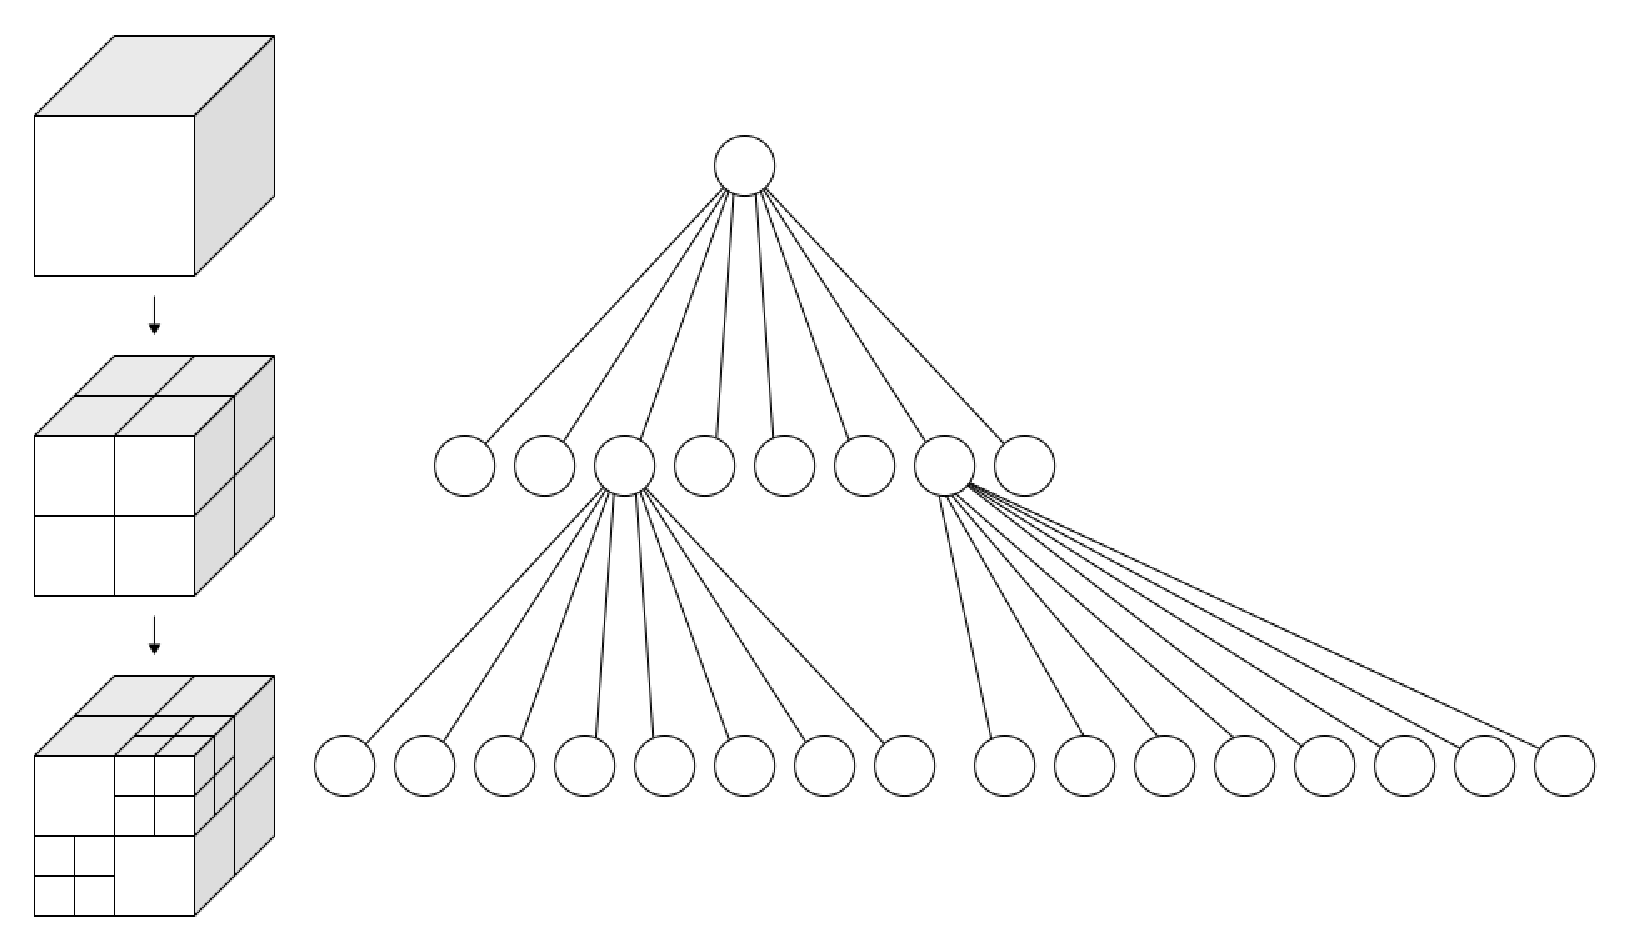
\includegraphics[width=0.8\textwidth]{octree.eps}}
\caption{Schéma de décomposition d'un octree}
\label{octree_img}
\end{figure}

\paragraph{}
Après sous-division, les objets sont éparpillés dans les cubes enfants en
fonction de leur position dans l'espace. Il s'agit, pour simplifier, de classer
les objets via une sorte de dichotomie pour chaque dimension, d'où les 8 cubes.
La recherche d'un élément via ses coordonnées est alors très rapide, puisque
les éléments sont disposés dans chaque cube en fonction de cette variable.


\subsubsection{Recherche de voisins}
\paragraph{}
Dans chaque cube, les éléments sont stockés dans une ArrayList de taille
maximum $M$, fixée et comprise entre 1 et $N$ ($N$ le nombre total d'éléments
stockés dans l'ensemble de l'octree). La recherche de voisins s'effectue en
cherchant les cubes entourant un objet. La recherche du plus proche voisin a
alors comme complexité dans le pire cas $O(27(M + N))$, soit environ $O(M+N)$.
$O(M)$ est ici la complexité à parcourir tous les éléments de chaque cube
(puisque cela revient à parcourir une ArrayList de taille $M$). $O(N)$
correspond à la complexité à atteindre un cube donné dans l'octree dans le pire
des cas. Ces deux complexités sont à multiplier par 27, qui correspond au
nombre maximum de cubes pouvant entourer un objet. Dans le cas où $M$ est fixée
à la même valeur que $N$, la complexité est de $O(2N)$ par atome, soit $O(N^2)$
pour avoir le plus proche voisin pour l'ensemble des $N$ atomes.

\paragraph{}
Le cas moyen est intéressant à étudier car montre le rôle que joue M dans
l'efficacité de l'algorithme. La complexité est de $O(M +
\frac{\log(N)}{3\log(M)\times{}\log(2)})$, soit environ $O(M +
\frac{\log(N)}{\log(M)})$. On négligera le nombre de cubes entourant l'élément
puisqu'il n'impacte que peu la complexité finale. $O(M)$ est ici encore la
complexité à parcourir tous les éléments d'un cube (ArrayList de taille $M$).
$O(\frac{\log(N)}{\log(M)})$ correspond ici à la complexité d'accéder à un cube
donné. Le nombre de cubes moyen entourant un objet est ici négligé. Si $M$ se
rapproche de 1, la complexité est environ de $O(N)$ par atome, soit $O(N^2)$
pour l'ensemble des atomes. La complexité est environ la même si $M = N$.
Néanmoins, il est plus avantageux que $M$ soit égal à $N$ plutôt qu'à 1, à
cause du nombre de cubes entourant l'objet pas mis en évidence ici car non pris
en compte dans les calculs.

\paragraph{}
On s'aperçoit alors que l'Octree est avantageux pour la recherche de voisins,
mais il est important de fixer une valeur appropriée pour le nombre maximum
d'éléments par cube, auquel cas la complexité sera plus mauvaise que celle
d'une ArrayList. Fixer un $M$ trop faible reviendra à obtenir énormément de
cubes, puisqu'un cube ne pourra contenir que peu d'éléments, ce qui rendra lent
l'accès à un cube donné. Fixer un $M$ trop proche de $N$ rendra l'octree
inefficace, car sera composé de très peu de cubes contenant un grand nombre
d'éléments.


\subsubsection{Déplacement d'éléments}
\paragraph{}
Les nœuds de l'arbre dépendent des coordonnées des points, donc déplacer un
point peut amener à déplacer un nœud. Contrairement à l'arbre k-d, cette étape
n'est pas forcément nécessaire, et le déplacement léger d'un atome ne
requièrera pas, dans la plupart des cas, d'être déplacé dans un autre cube.  On
aura alors dans la plupart des cas une complexité de $O(1)$ pour le déplacement
d'un atome, et au pire $O(N)$ ($O(2N)$ pour accéder au cube de l'élément à
déplacer puis le supprimer de l'ArrayList, $O(2N)$ pour l'insérer dans le cube
approprié à ses nouvelles coordonnées). Également, un octree n'a pas besoin
d'être équilibré. Ces deux points en font un arbre intéressant pour le cas de
la simulation d'atomes, où les éléments sont sans cesse en mouvement.


\subsubsection{Choisi comme datastructure principale}
\paragraph{}
L'octree a été choisi comme datastructure servant à stocker ses atomes pour sa
facilité d'implémentation comparé à un arbre k-d, la rapidité en moyenne à
déplacer un élément et la complexité de la recherche de voisin le plus proche,
qui permet d'être au pire quasiment aussi efficace qu'une ArrayList, et dans le
meilleur des cas permet de se rapproche d'une complexité en $O(\log(N))$ par
élément, soit $O(N\log(N))$ pour l'ensemble des atomes, lorsque la variable $M$
est correctement fixée et $N$ assez grand.

\subsection{K-D Tree}

\paragraph{}
Un K-D tree est un arbre binaire, équilibré. La complexité en cas moyen pour de
la recherche de voisins est de $O(log(N))$, pire cas $O(N)$. Comme pour
l'octree, les nœuds de l'arbre dépendent des coordonnées des points, donc ici
déplacer un point revient à déplacer un nœud et à re-balancer l'arbre. Ce point
est important car nous sommes ici dans un environnement où les atomes sont
constamment en mouvement.  La complexité d'insertion d'élément est en moyenne
de $O(log(N))$, ce qui est également le cas pour la suppression. Bouger un
élément dans l'arbre a alors une complexité de $O(2log(N))$.

\paragraph{}
Pour chaque frame, en cas moyen, la méthode de recherche de voisin ainsi que le
déplacement d'atome aurait une complexité de $O(3log(N))$, et comme pire cas
$O(3N)$. Au total, pour tous les atomes, la complexité totale serait alors de
$O(Nlog(N))$ en cas moyen et $O(N^2)$ en pire cas. Cela reste inférieur à la
complexité de l'ArrayList en cas moyen, mais il faut atteindre un grand nombre
d'atomes pour que la différence soit intéressante, c'est pourquoi la solution
n'a pas été retenue.
